\section{System Design}

\subsection{User Journeys}

\subsubsection{Client Journey}

\bigskip

\begin{figure}[H]
    \centering
    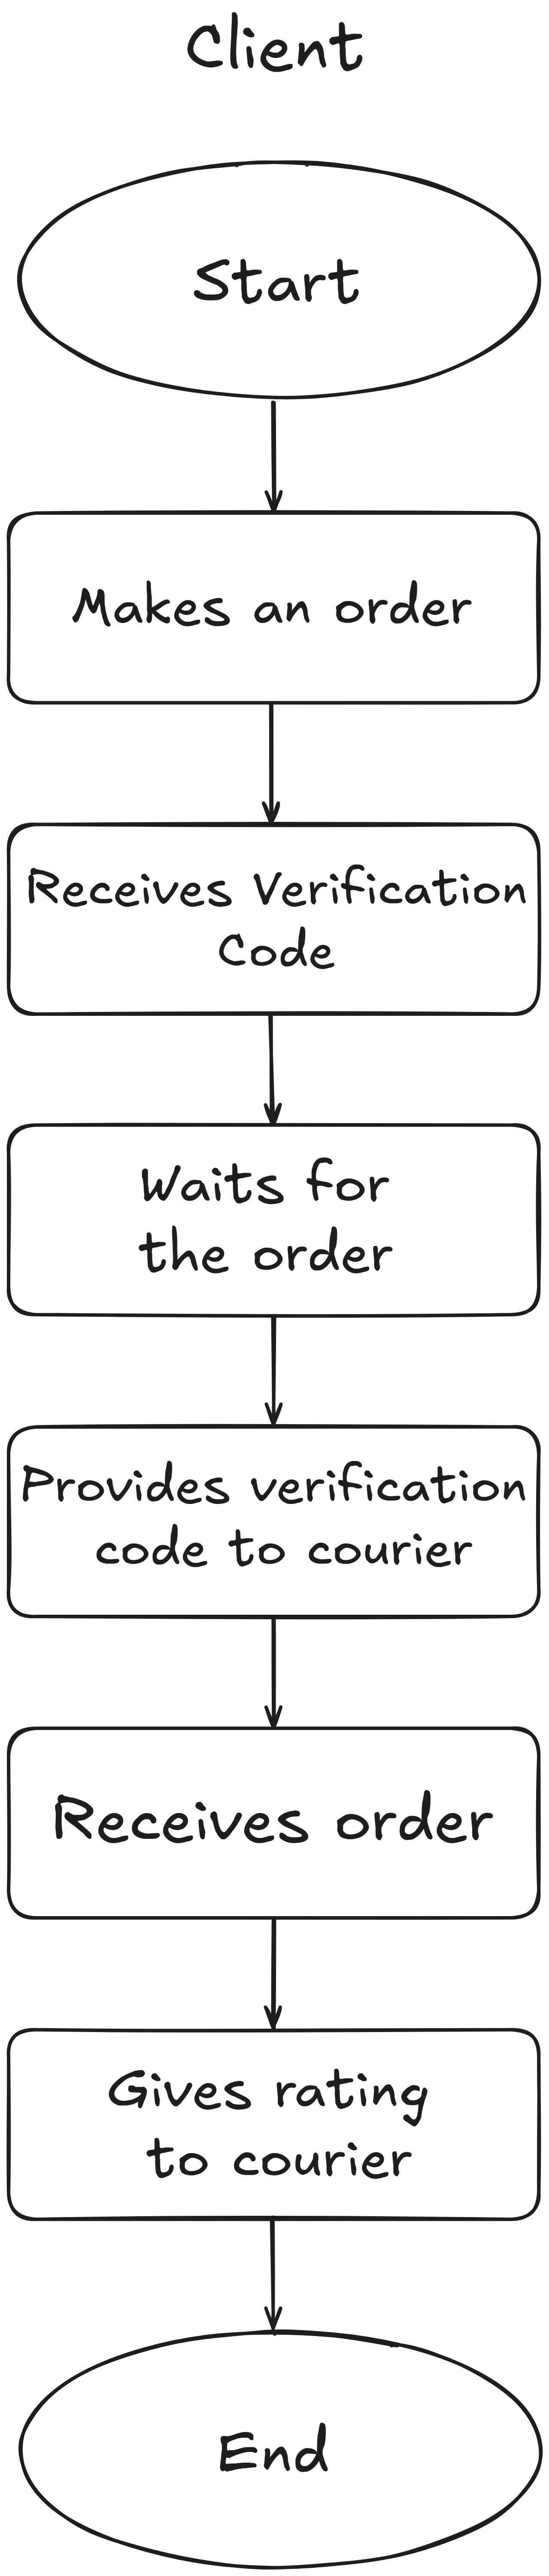
\includegraphics[width=0.2\textwidth]{images/ClientJourney.png} % adjust path & width if needed
    \caption{Client journey flowchart showing from the beginning}
    \label{fig:client_journey}
\end{figure}

This flowchart (\ref{fig:client_journey}) illustrates the sequential steps a client undergoes when placing an order through the LiftDrop platform. The process begins with the client initiating an order, followed by a waiting period for the order to be processed and accepted by a courier. Once the order is received, the client provides a unique confirmation code to the courier, marking a secure handoff. Finally, the process concludes with the client rating the delivery experience.

\newpage

\subsubsection{Courier Journey}

\bigskip

\begin{figure}[H]
    \centering
    \includegraphics[width=0.37\textwidth]{images/CourierJourney.png} % adjust path & width if needed
    \caption{Courier journey flowchart showing from the beginning}
    \label{fig:courier_journey}
\end{figure}

This flowchart (\ref{fig:courier_journey}) outlines the step-by-step decision-making process a courier follows while managing delivery requests on the LiftDrop platform. It begins with the courier awaiting an incoming order, which can either be accepted or rejected. Upon accepting a request, the courier proceeds to the pickup location, with the option to cancel if necessary. After pickup, the courier advances to the delivery phase. If the courier successfully reaches the destination, the delivery is confirmed. If the destination is not reached, the system prompts reevaluation or cancellation.

\newpage

\vspace{2mm}

\subsection{Interface Design}

The LiftDrop application includes distinct UI flows that guide couriers through each stage of the delivery lifecycle. This section presents key interface screens, organized by functionality and user context.

%\newpage

\subsubsection{Authentication Flow}

The authentication flow allows users to securely access the platform through account registration and login.

\begin{figure}[H]
    \centering
    \begin{subfigure}[b]{0.44\textwidth}
        \centering
        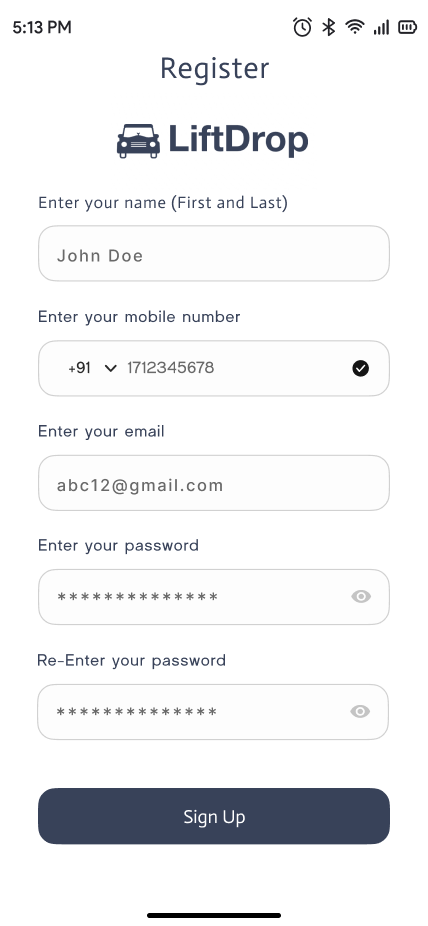
\includegraphics[width=\textwidth]{images/registration.png}
        \caption{User registration screen}
        \label{fig:registration}
    \end{subfigure}
    \hfill
    \begin{subfigure}[b]{0.44\textwidth}
        \centering
        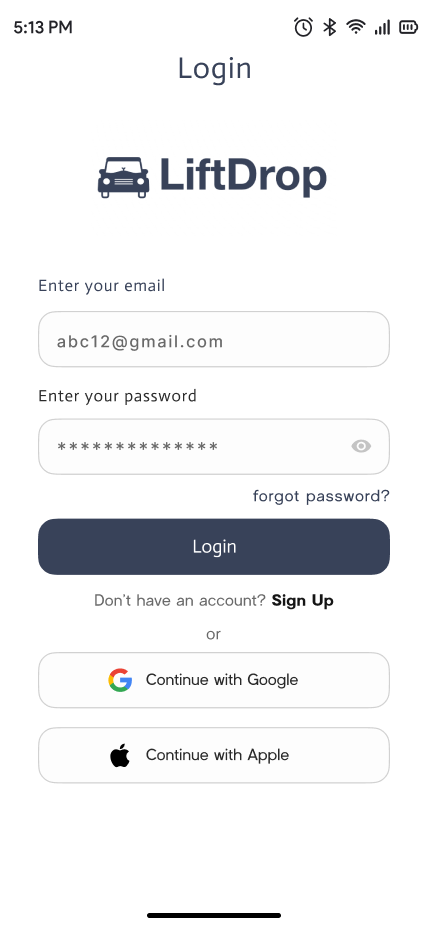
\includegraphics[width=\textwidth]{images/login.png}
        \caption{User login screen}
        \label{fig:login}
    \end{subfigure}
    \caption{Authentication flow screens in LiftDrop}
    \label{fig:auth_flow}
\end{figure}

\noindent\textbf{Registration Screen (\ref{fig:registration}):}  
Enables users to create an account by providing their name, email, and password.

\noindent\textbf{Login Screen (\ref{fig:login}):}  
Provides a simple interface for returning users to log in with their credentials.

\subsubsection{Courier Flow}

The following screens illustrate the courier experience—from going online to completing a delivery.

\begin{figure}[H]
    \centering
    \begin{subfigure}[b]{0.48\textwidth}
        \centering
        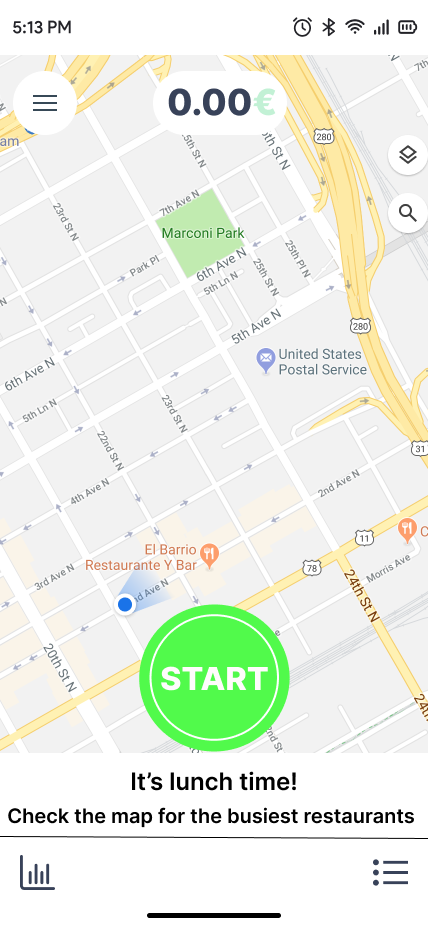
\includegraphics[width=\textwidth]{images/go_screen.png}
        \caption{Idle status screen}
        \label{fig:go_screen}
    \end{subfigure}
    \hfill
    \begin{subfigure}[b]{0.48\textwidth}
        \centering
        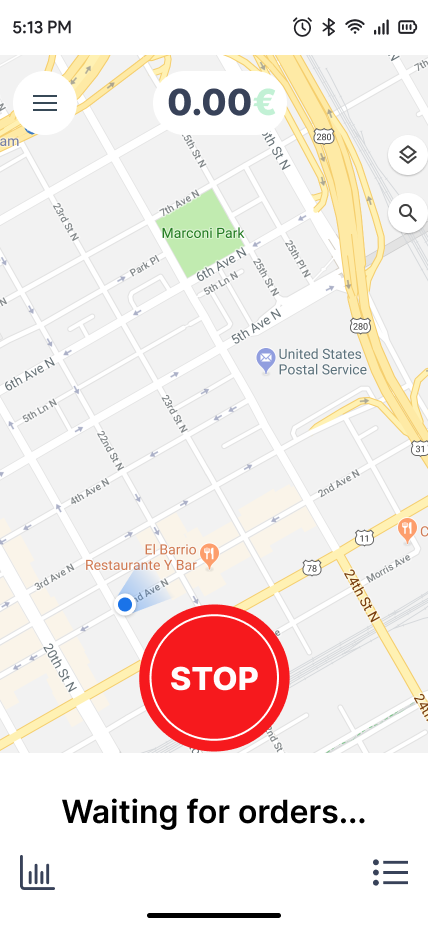
\includegraphics[width=\textwidth]{images/waiting_screen.png}
        \caption{Waiting for order screen}
        \label{fig:waiting_screen}
    \end{subfigure}
    \caption{Courier status screens during online session}
    \label{fig:courier_status}
\end{figure}

\noindent\textbf{Idle Screen (\ref{fig:go_screen}):}  
Allows couriers to toggle availability and begin accepting orders.

\noindent\textbf{Waiting Screen (\ref{fig:waiting_screen}):}  
Indicates that the system is searching for nearby orders in real time.

\begin{figure}[H]
    \centering
    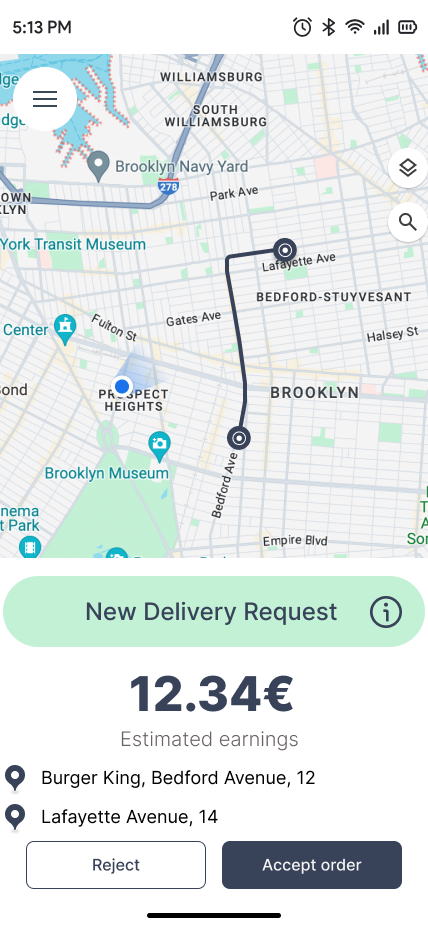
\includegraphics[width=0.6\textwidth]{images/delivery_request.png}
    \caption{Incoming delivery request with order summary and action buttons}
    \label{fig:delivery_request}
\end{figure}

\noindent\textbf{Delivery Request (\ref{fig:delivery_request}):}  
Displays order metadata such as pickup and drop-off addresses, delivery distance, and quick actions to accept or decline.

\begin{figure}[H]
    \centering
    \begin{subfigure}[b]{0.48\textwidth}
        \centering
        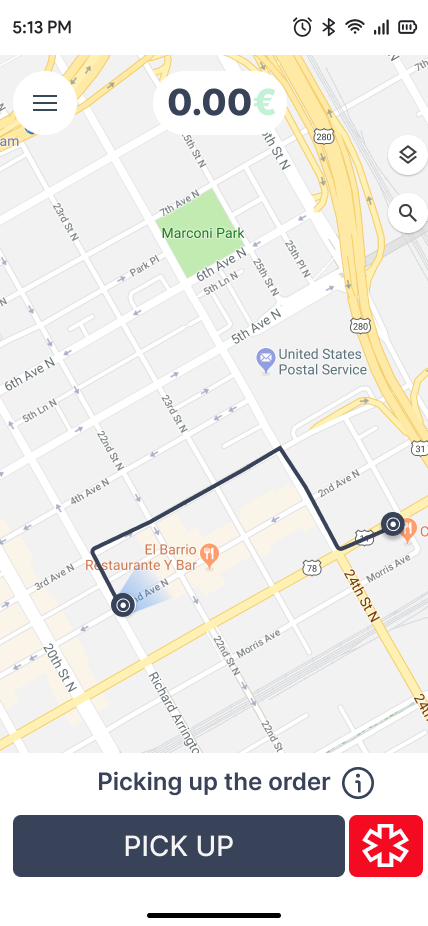
\includegraphics[width=\textwidth]{images/pickup_order_screen.png}
        \caption{Pickup confirmation screen}
        \label{fig:pickup_order}
    \end{subfigure}
    \hfill
    \begin{subfigure}[b]{0.48\textwidth}
        \centering
        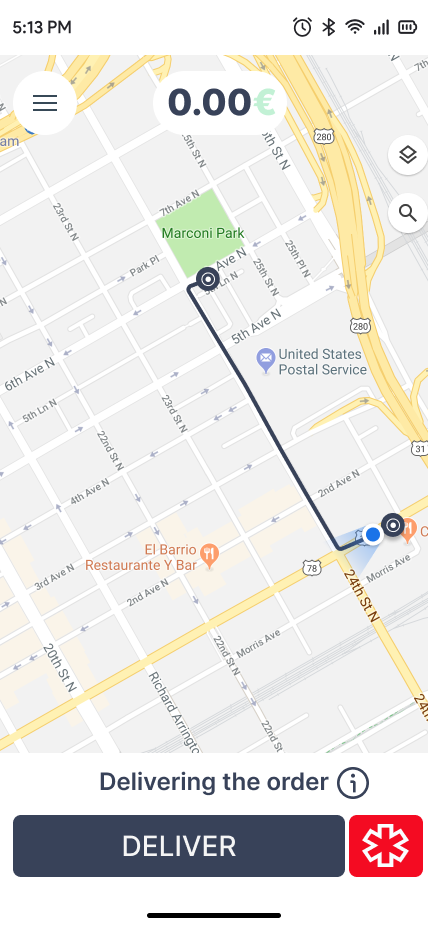
\includegraphics[width=\textwidth]{images/deliver_order_screen.png}
        \caption{Delivery confirmation screen}
        \label{fig:deliver_order}
    \end{subfigure}
    \caption{Screens for confirming pickup and delivery}
    \label{fig:courier_pickup_deliver}
\end{figure}

\noindent\textbf{Pickup Screen (\ref{fig:pickup_order}):}  
Guides the courier to confirm pickup, with cancelation support and verification of PIN.

\noindent\textbf{Delivery Screen (\ref{fig:deliver_order}):}  
Guides the courier to confirm delivery, with cancelation support and verification of PIN.

\newpage

\subsection{System Architecture and Data Model}

This section presents different architectural perspectives of the LiftDrop system, including component-level interactions and data model relationships. Each view emphasizes a specific aspect of the system's behavior, from geolocation handling to user roles and delivery lifecycle.

\subsubsection{High-Level System Architecture}

Figure~\ref{fig:high-level-Overview} illustrates the top-level architecture of the LiftDrop platform. It shows how the Android mobile application communicates with backend services responsible for order management, user interaction, real-time communication, and location processing.

\vspace{8mm}

\begin{figure}[H]
    \centering
    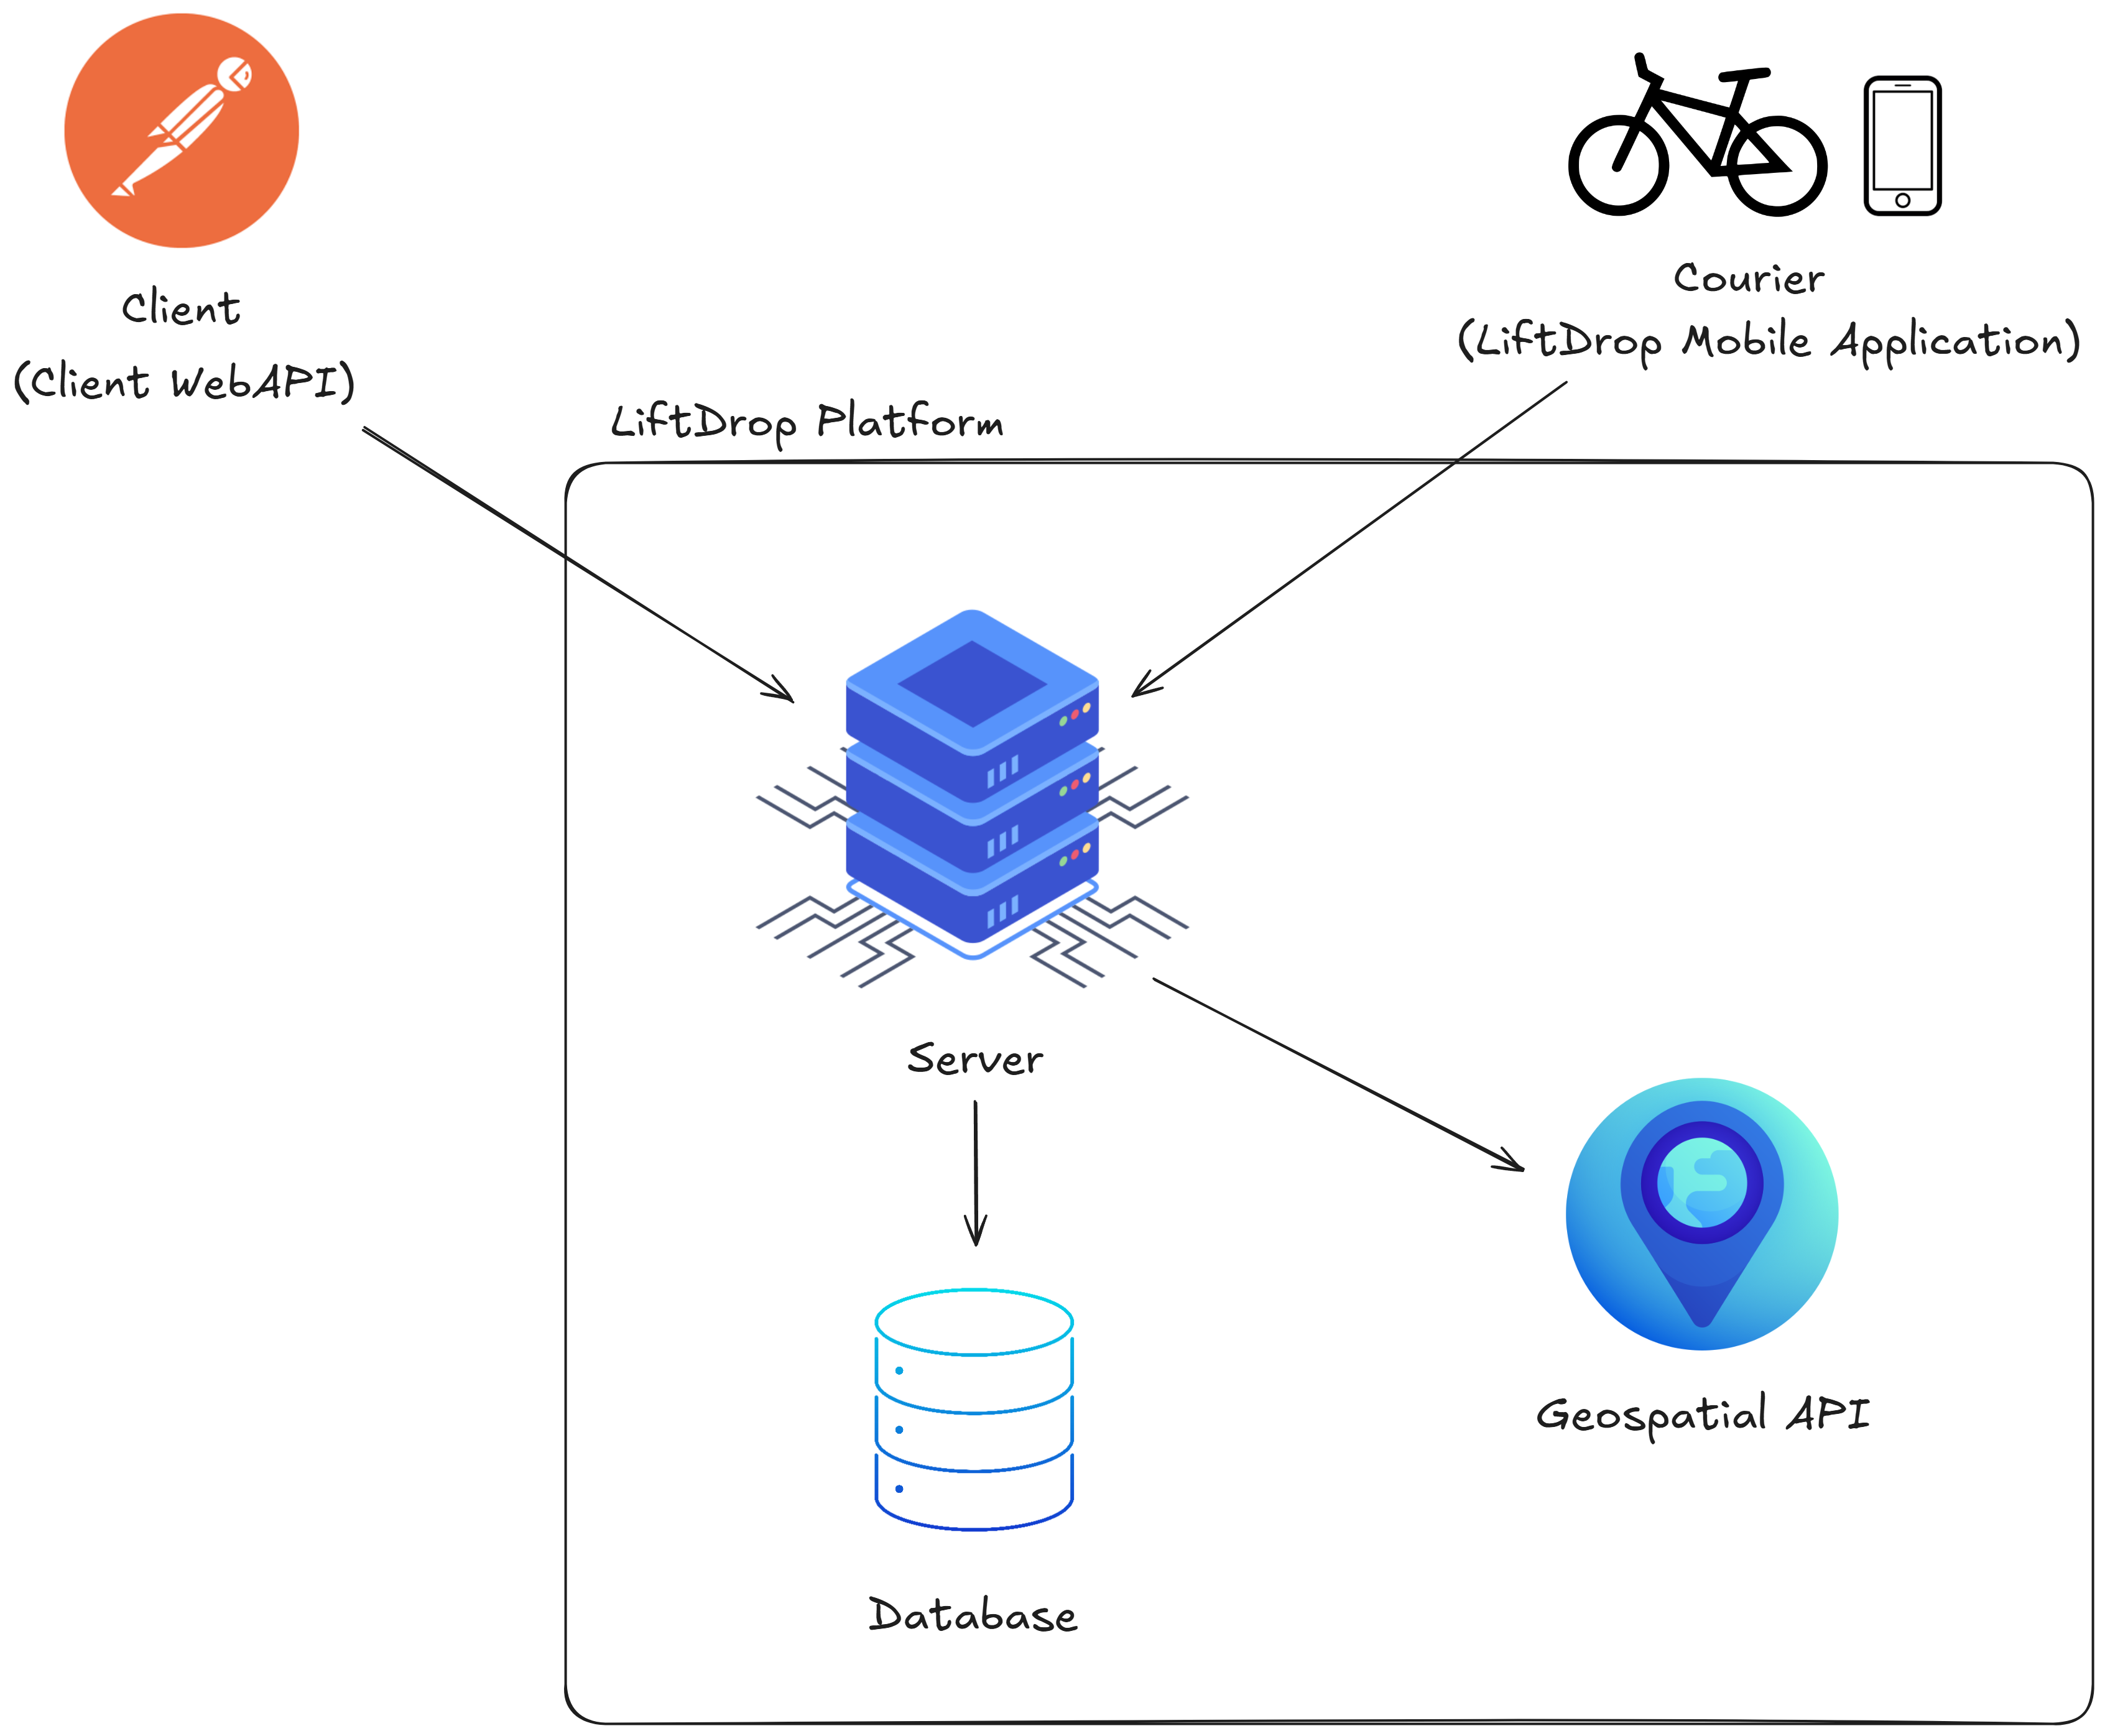
\includegraphics[width=0.82\textwidth]{images/LiftDrop_High_level_view.png}
    \caption{High-level overview of the LiftDrop system architecture}
    \label{fig:high-level-Overview}
\end{figure}

\newpage

\subsubsection{Location Model Overview}

This view isolates the system's handling of geospatial information. The \texttt{Location} class acts as a base abstraction for different types of spots used during a delivery. Specialized entities like \texttt{PickupSpot} and \texttt{DropOffSpot} inherit from \texttt{Location}, allowing consistent treatment of position data. A pickup spot can contain multiple \texttt{Item} entries, each identified by a unique designation.

\begin{figure}[H]
    \centering
    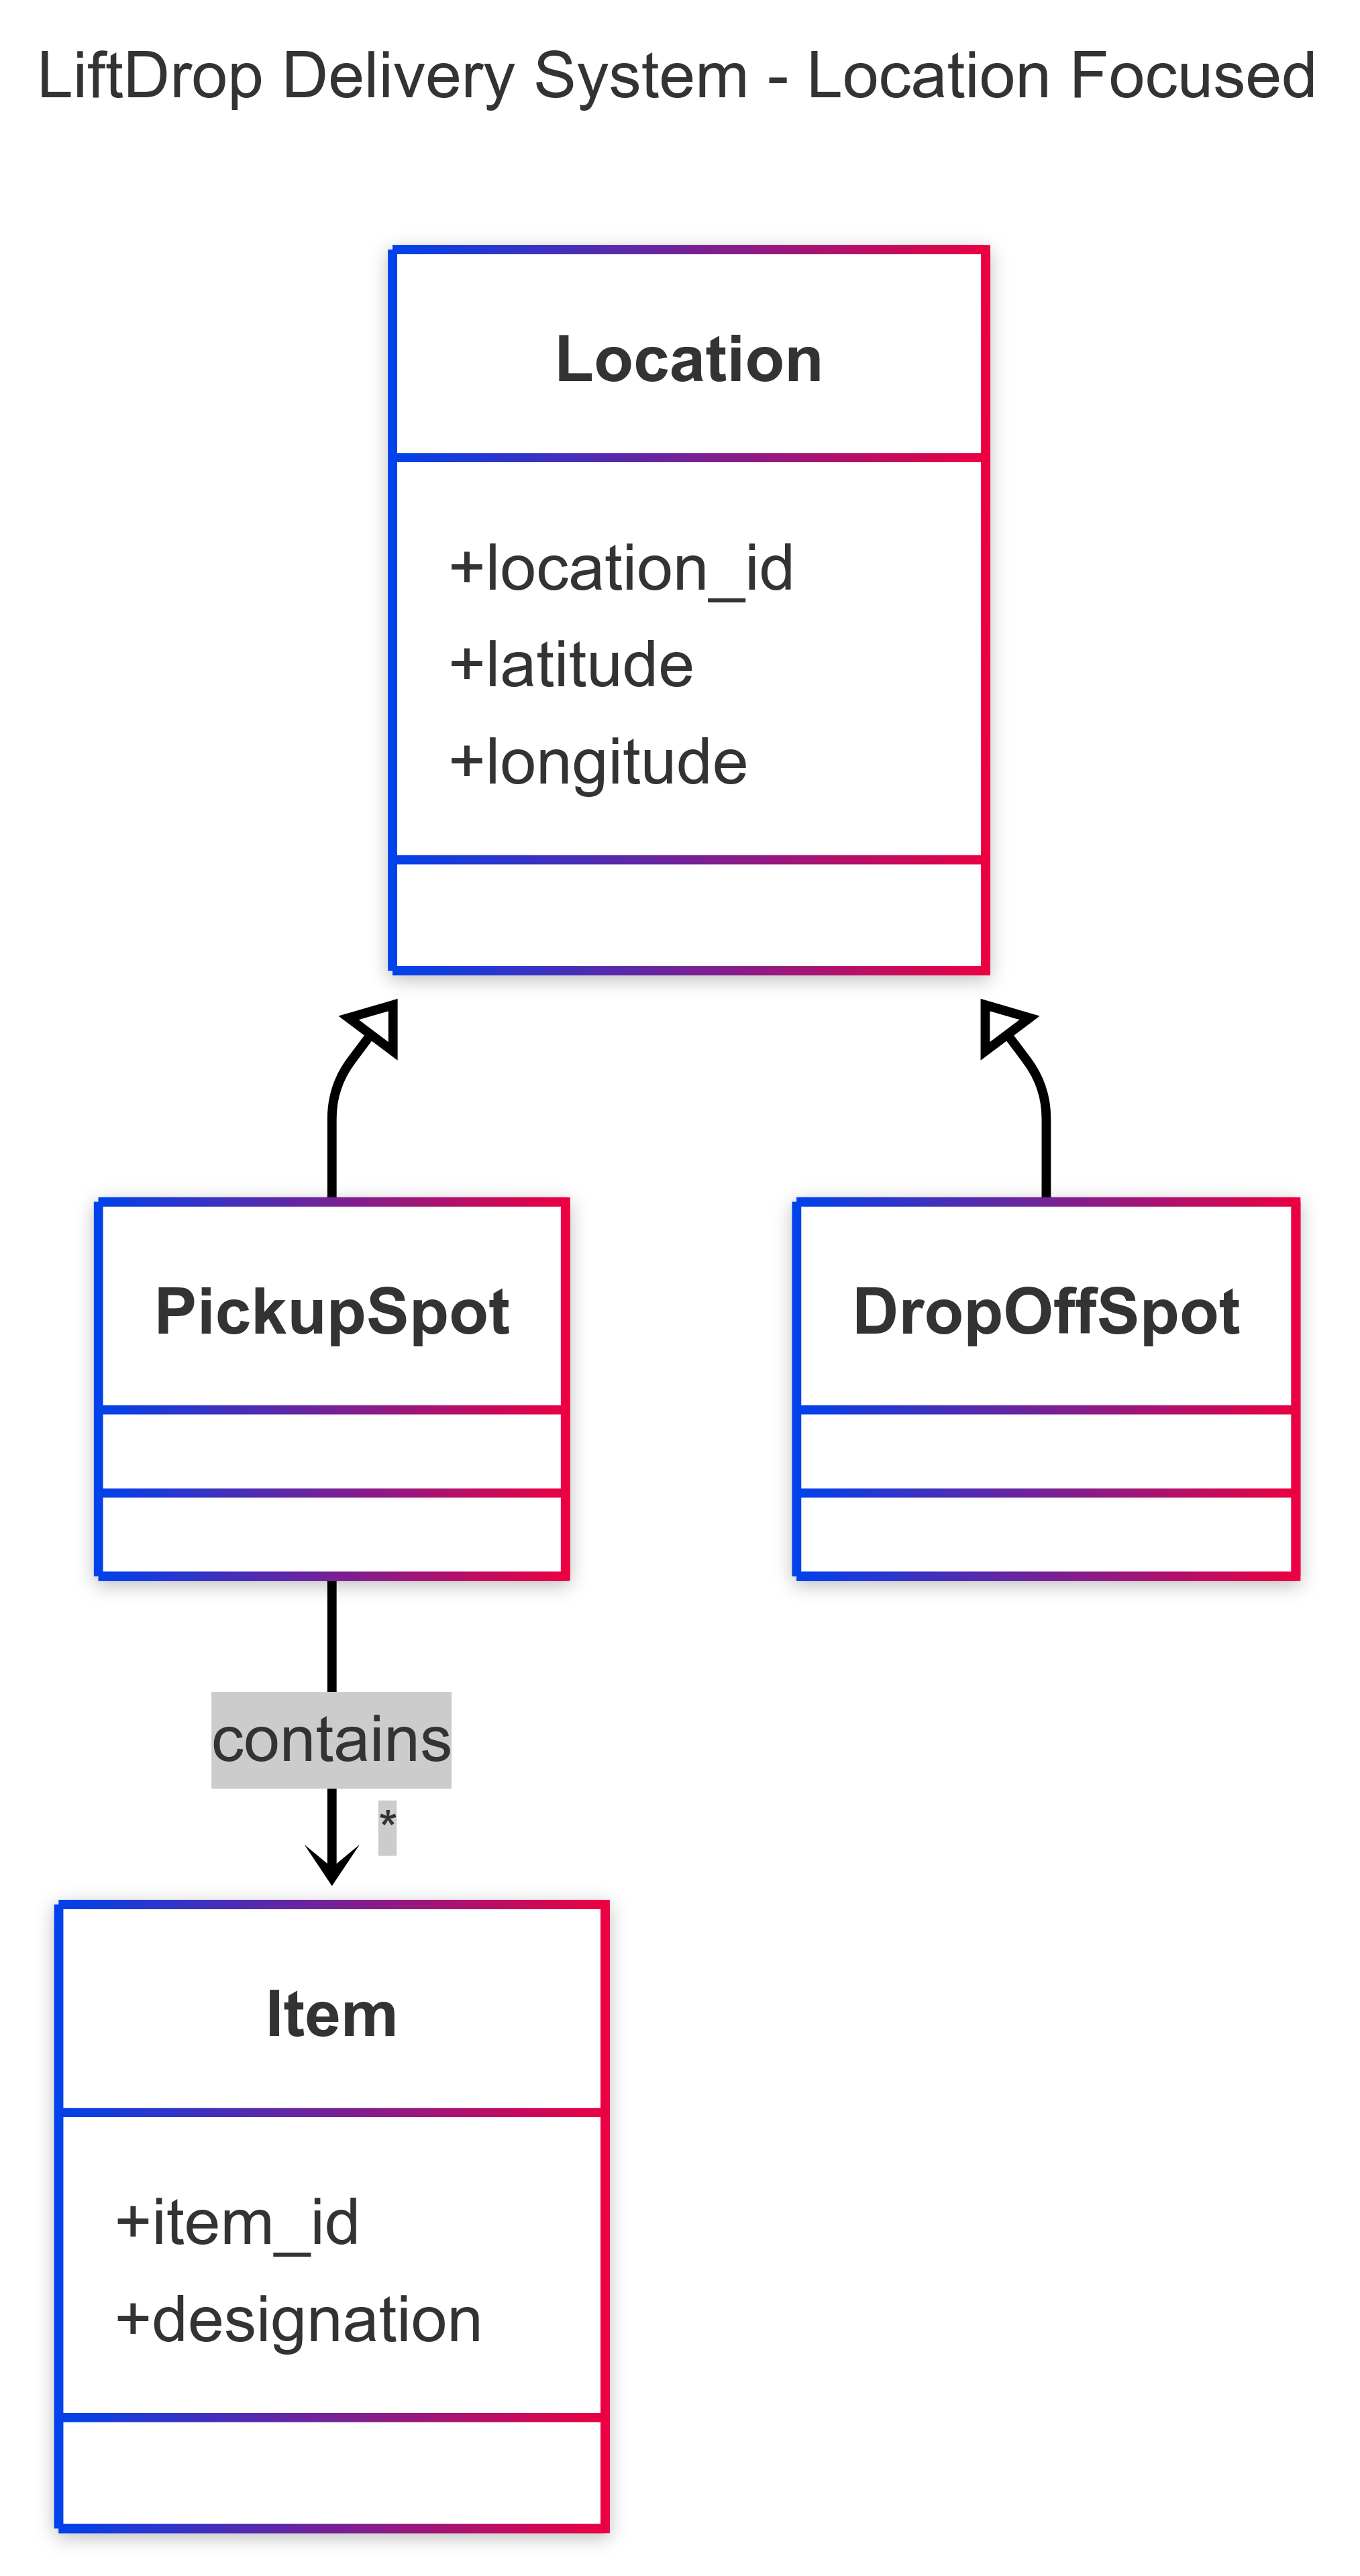
\includegraphics[width=0.44\textwidth]{images/LocationDiagram.png}
    \caption{Location Model Structure}
\end{figure}

\newpage

\subsubsection{User Role and Interaction Model}

This simplified diagram captures user roles and their interaction with delivery workflows. A \texttt{Client} can place multiple \texttt{Request}s, and a \texttt{Courier} can fulfill many of them. Each request is linked to a corresponding \texttt{Delivery}, forming a one-to-one mapping between a request and its fulfillment.
  
\begin{figure}[H]
    \centering
    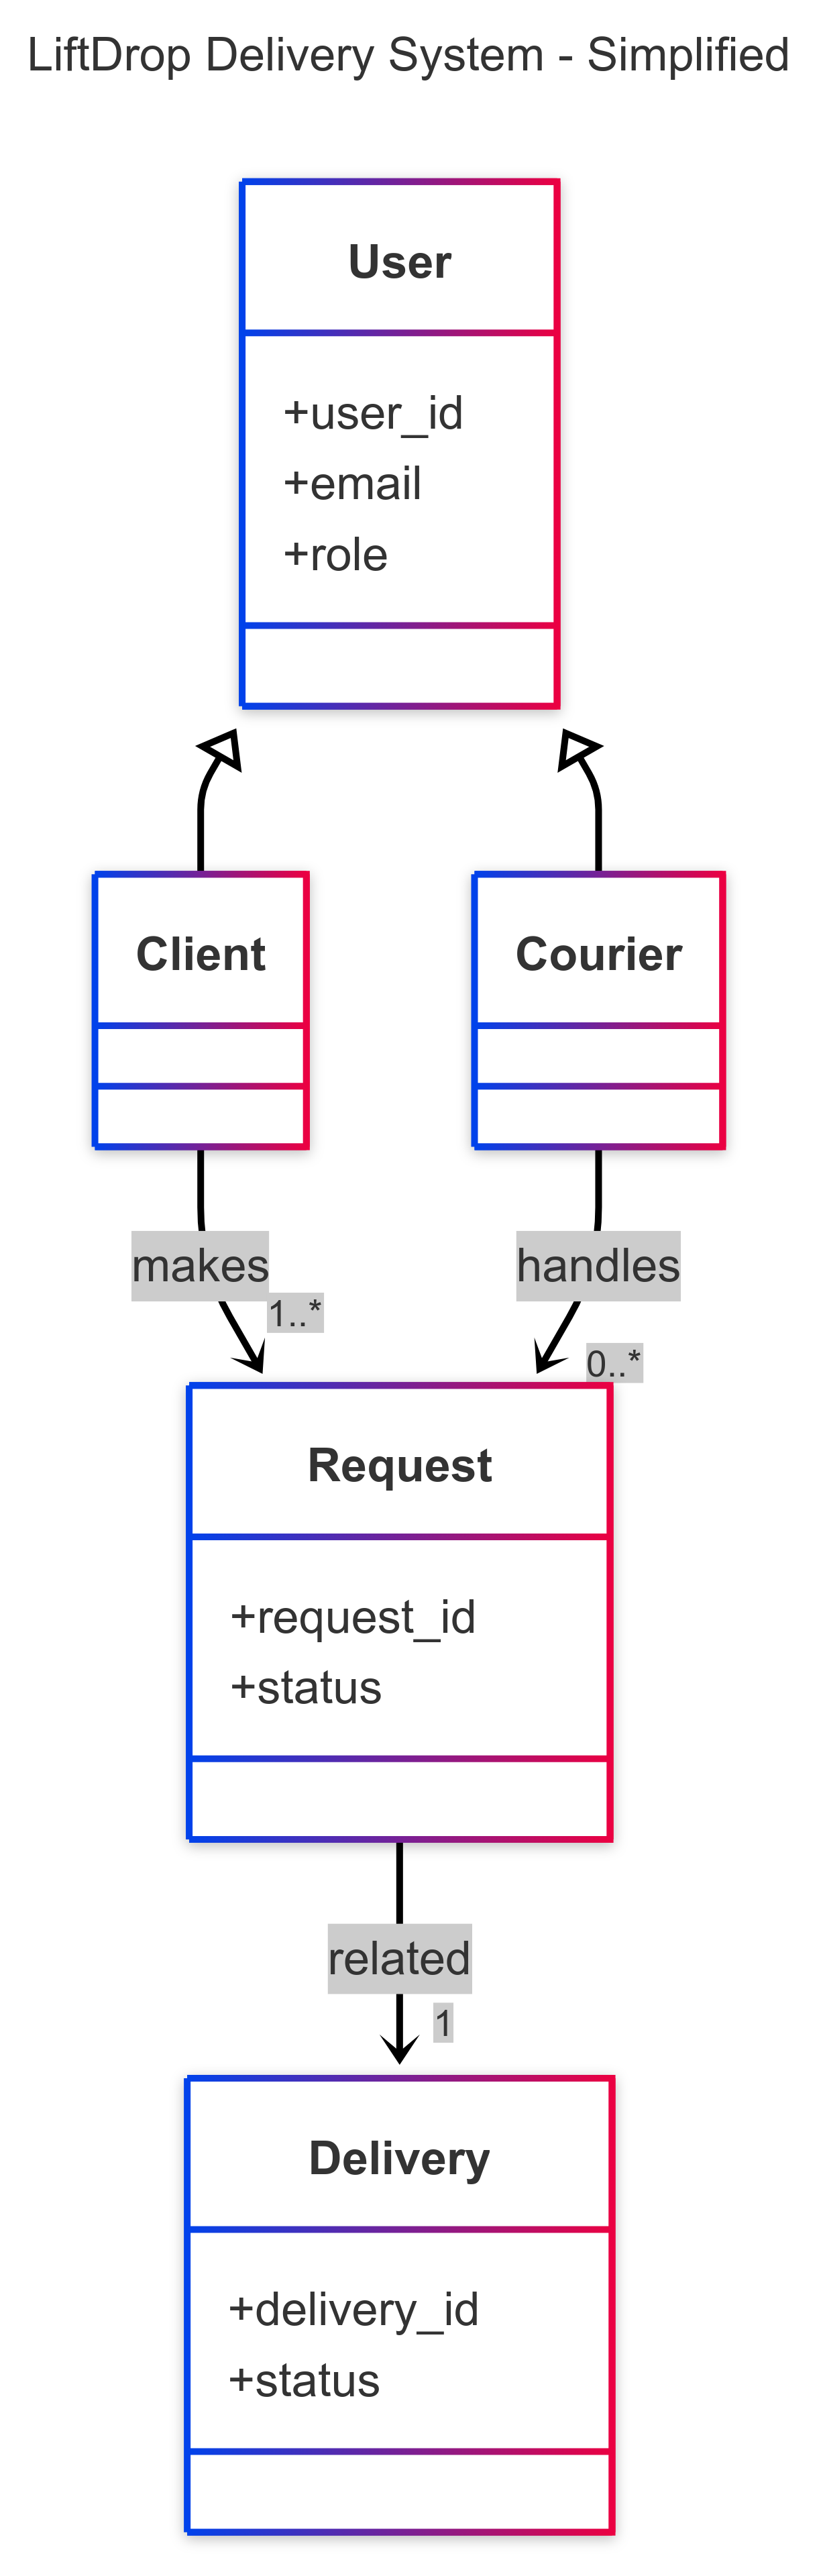
\includegraphics[width=0.40\textwidth]{images/UserClientCourierDiagram.png}
    \caption{User and Role Relationships}
\end{figure}

\subsubsection{Request and Delivery Lifecycle View}

This view focuses on how a request progresses through the system. Each \texttt{Request} includes additional metadata encapsulated in a \texttt{RequestDetails} object and is associated with a single \texttt{Delivery}. This structure supports clear traceability and separation of concerns between request creation and execution.

\begin{figure}[H]
    \centering
    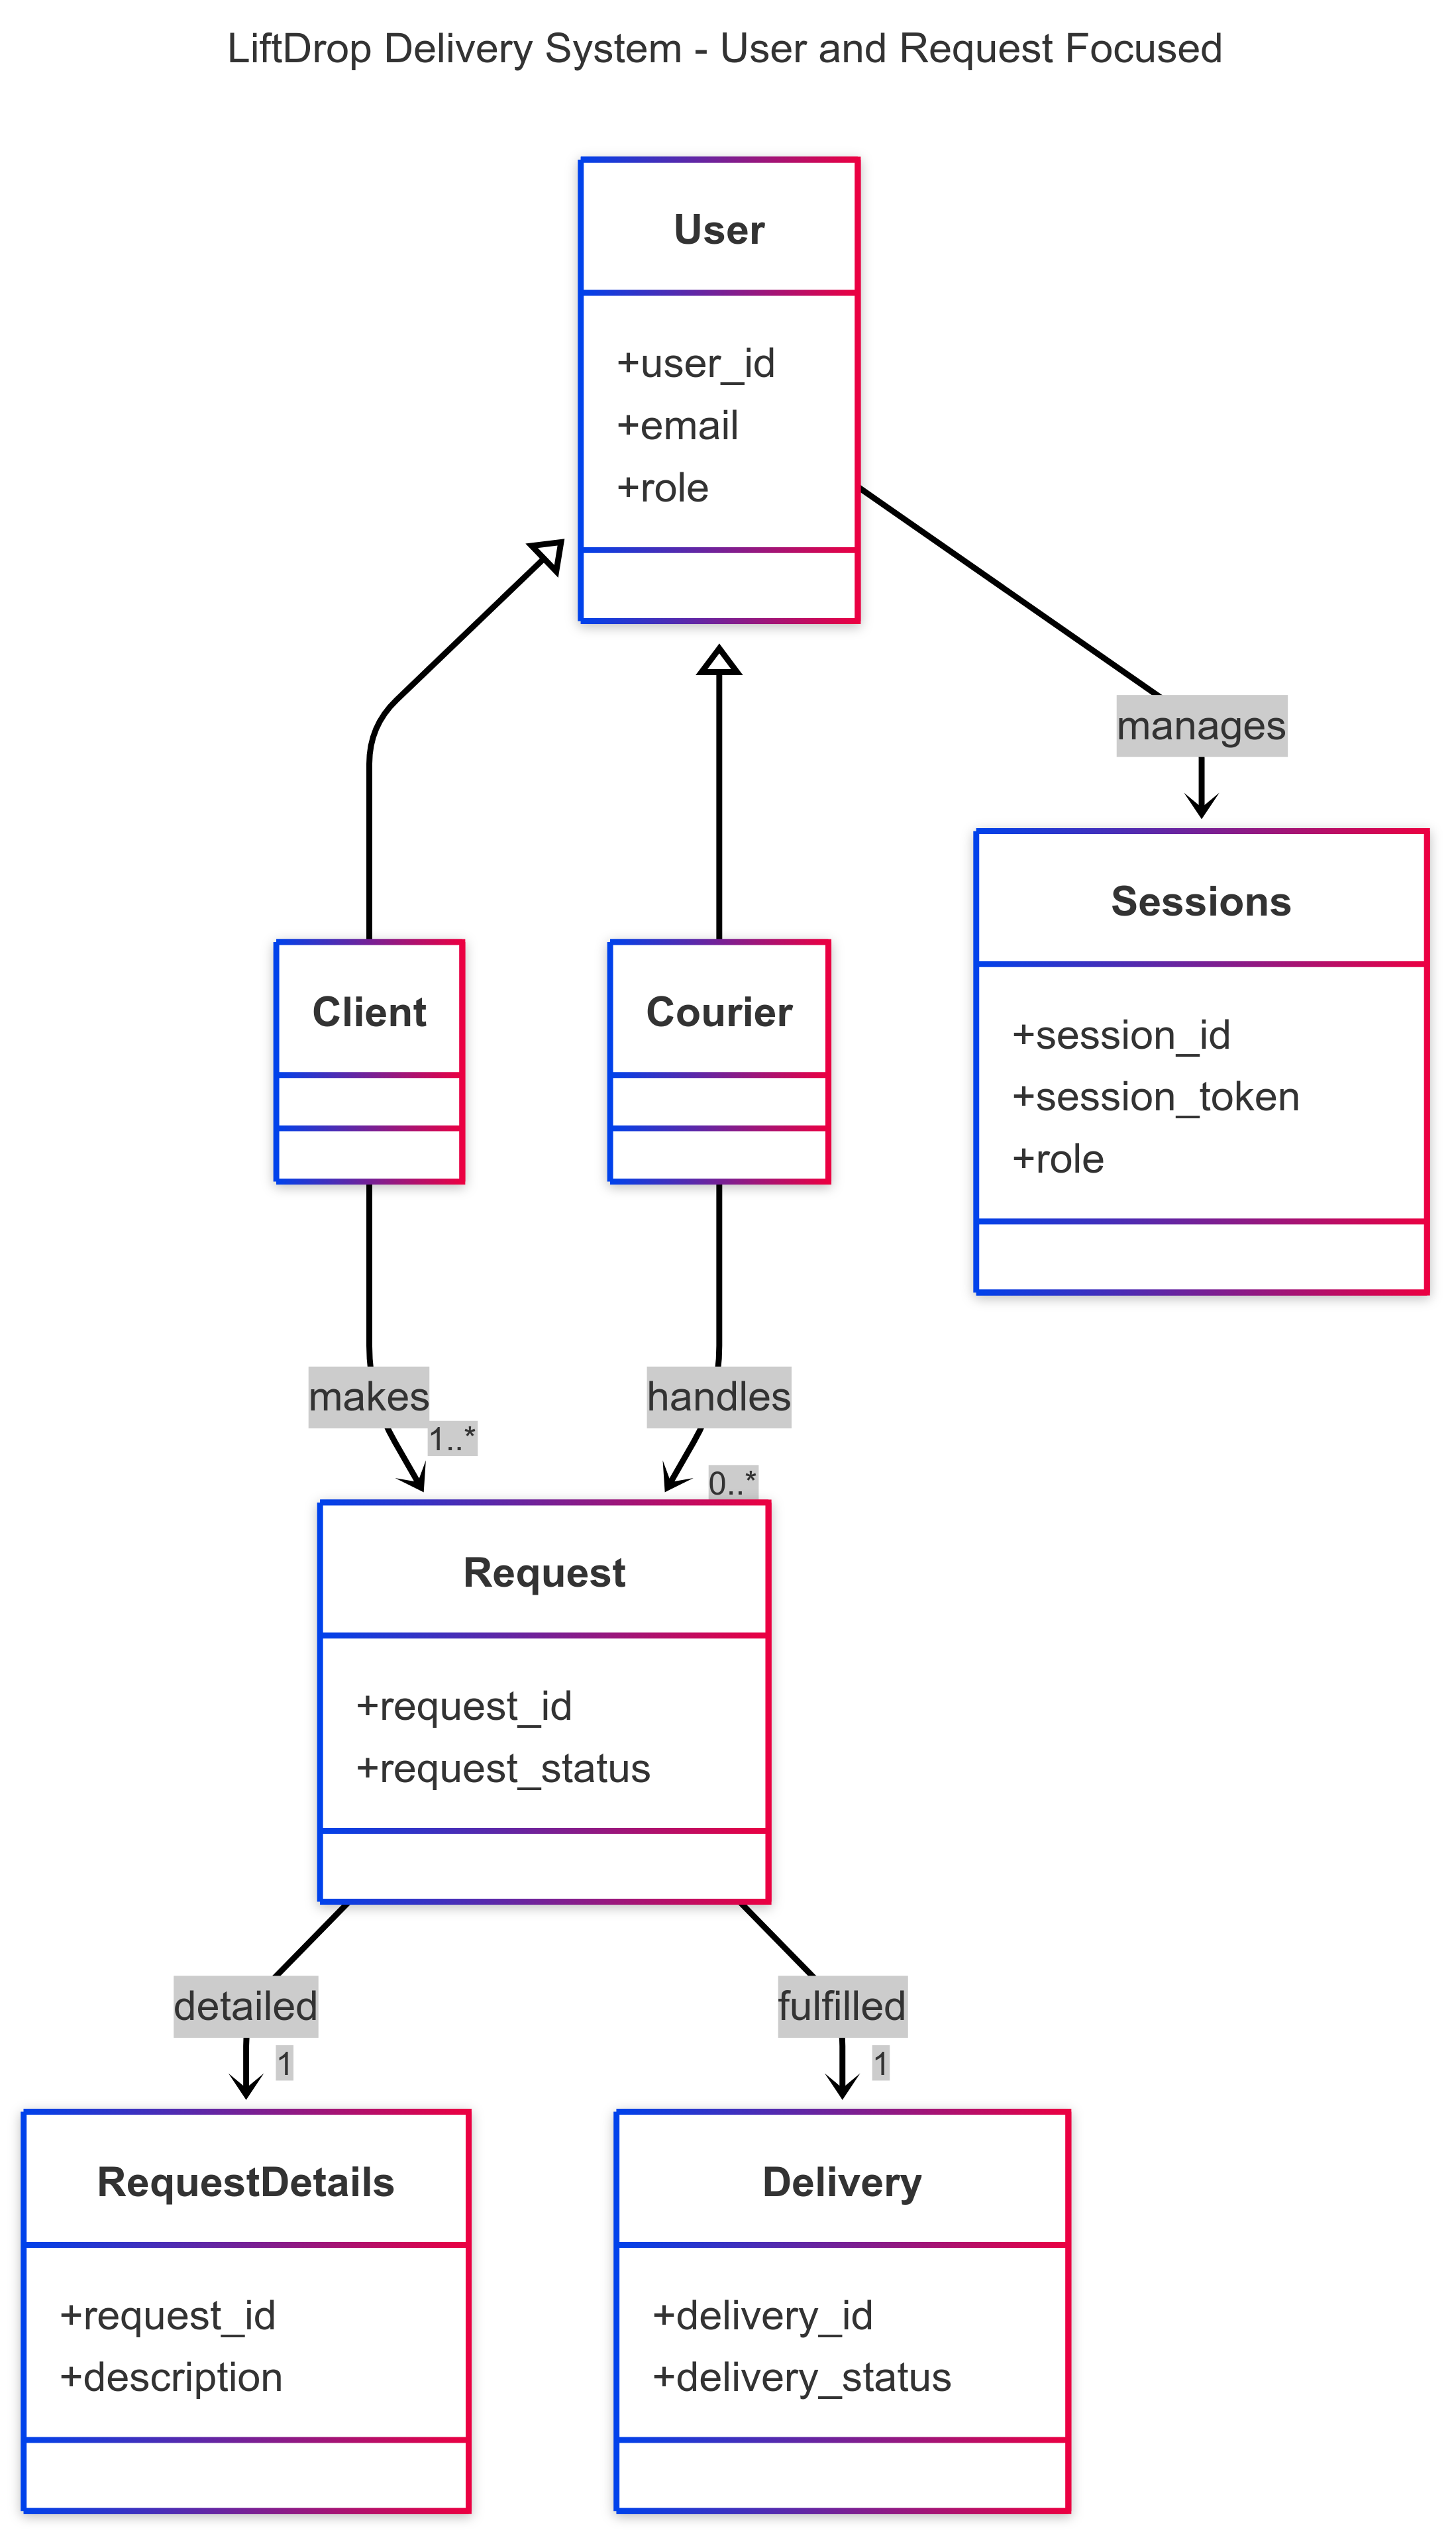
\includegraphics[width=0.44\textwidth]{images/UserSessions.png}
    \caption{Request and Fulfillment Architecture}
\end{figure}

\newpage

\subsubsection{Comprehensive System Model}

The complete data model integrates all key domain entities: \texttt{User}, \texttt{Address}, \texttt{Location}, \texttt{Item}, \texttt{Request}, \texttt{Delivery}, and \texttt{Session}. It captures how users interact with the system, how orders are structured and routed, and how real-time delivery coordination is maintained through geolocation and session-aware tracking.

\begin{figure}[H]
    \centering
    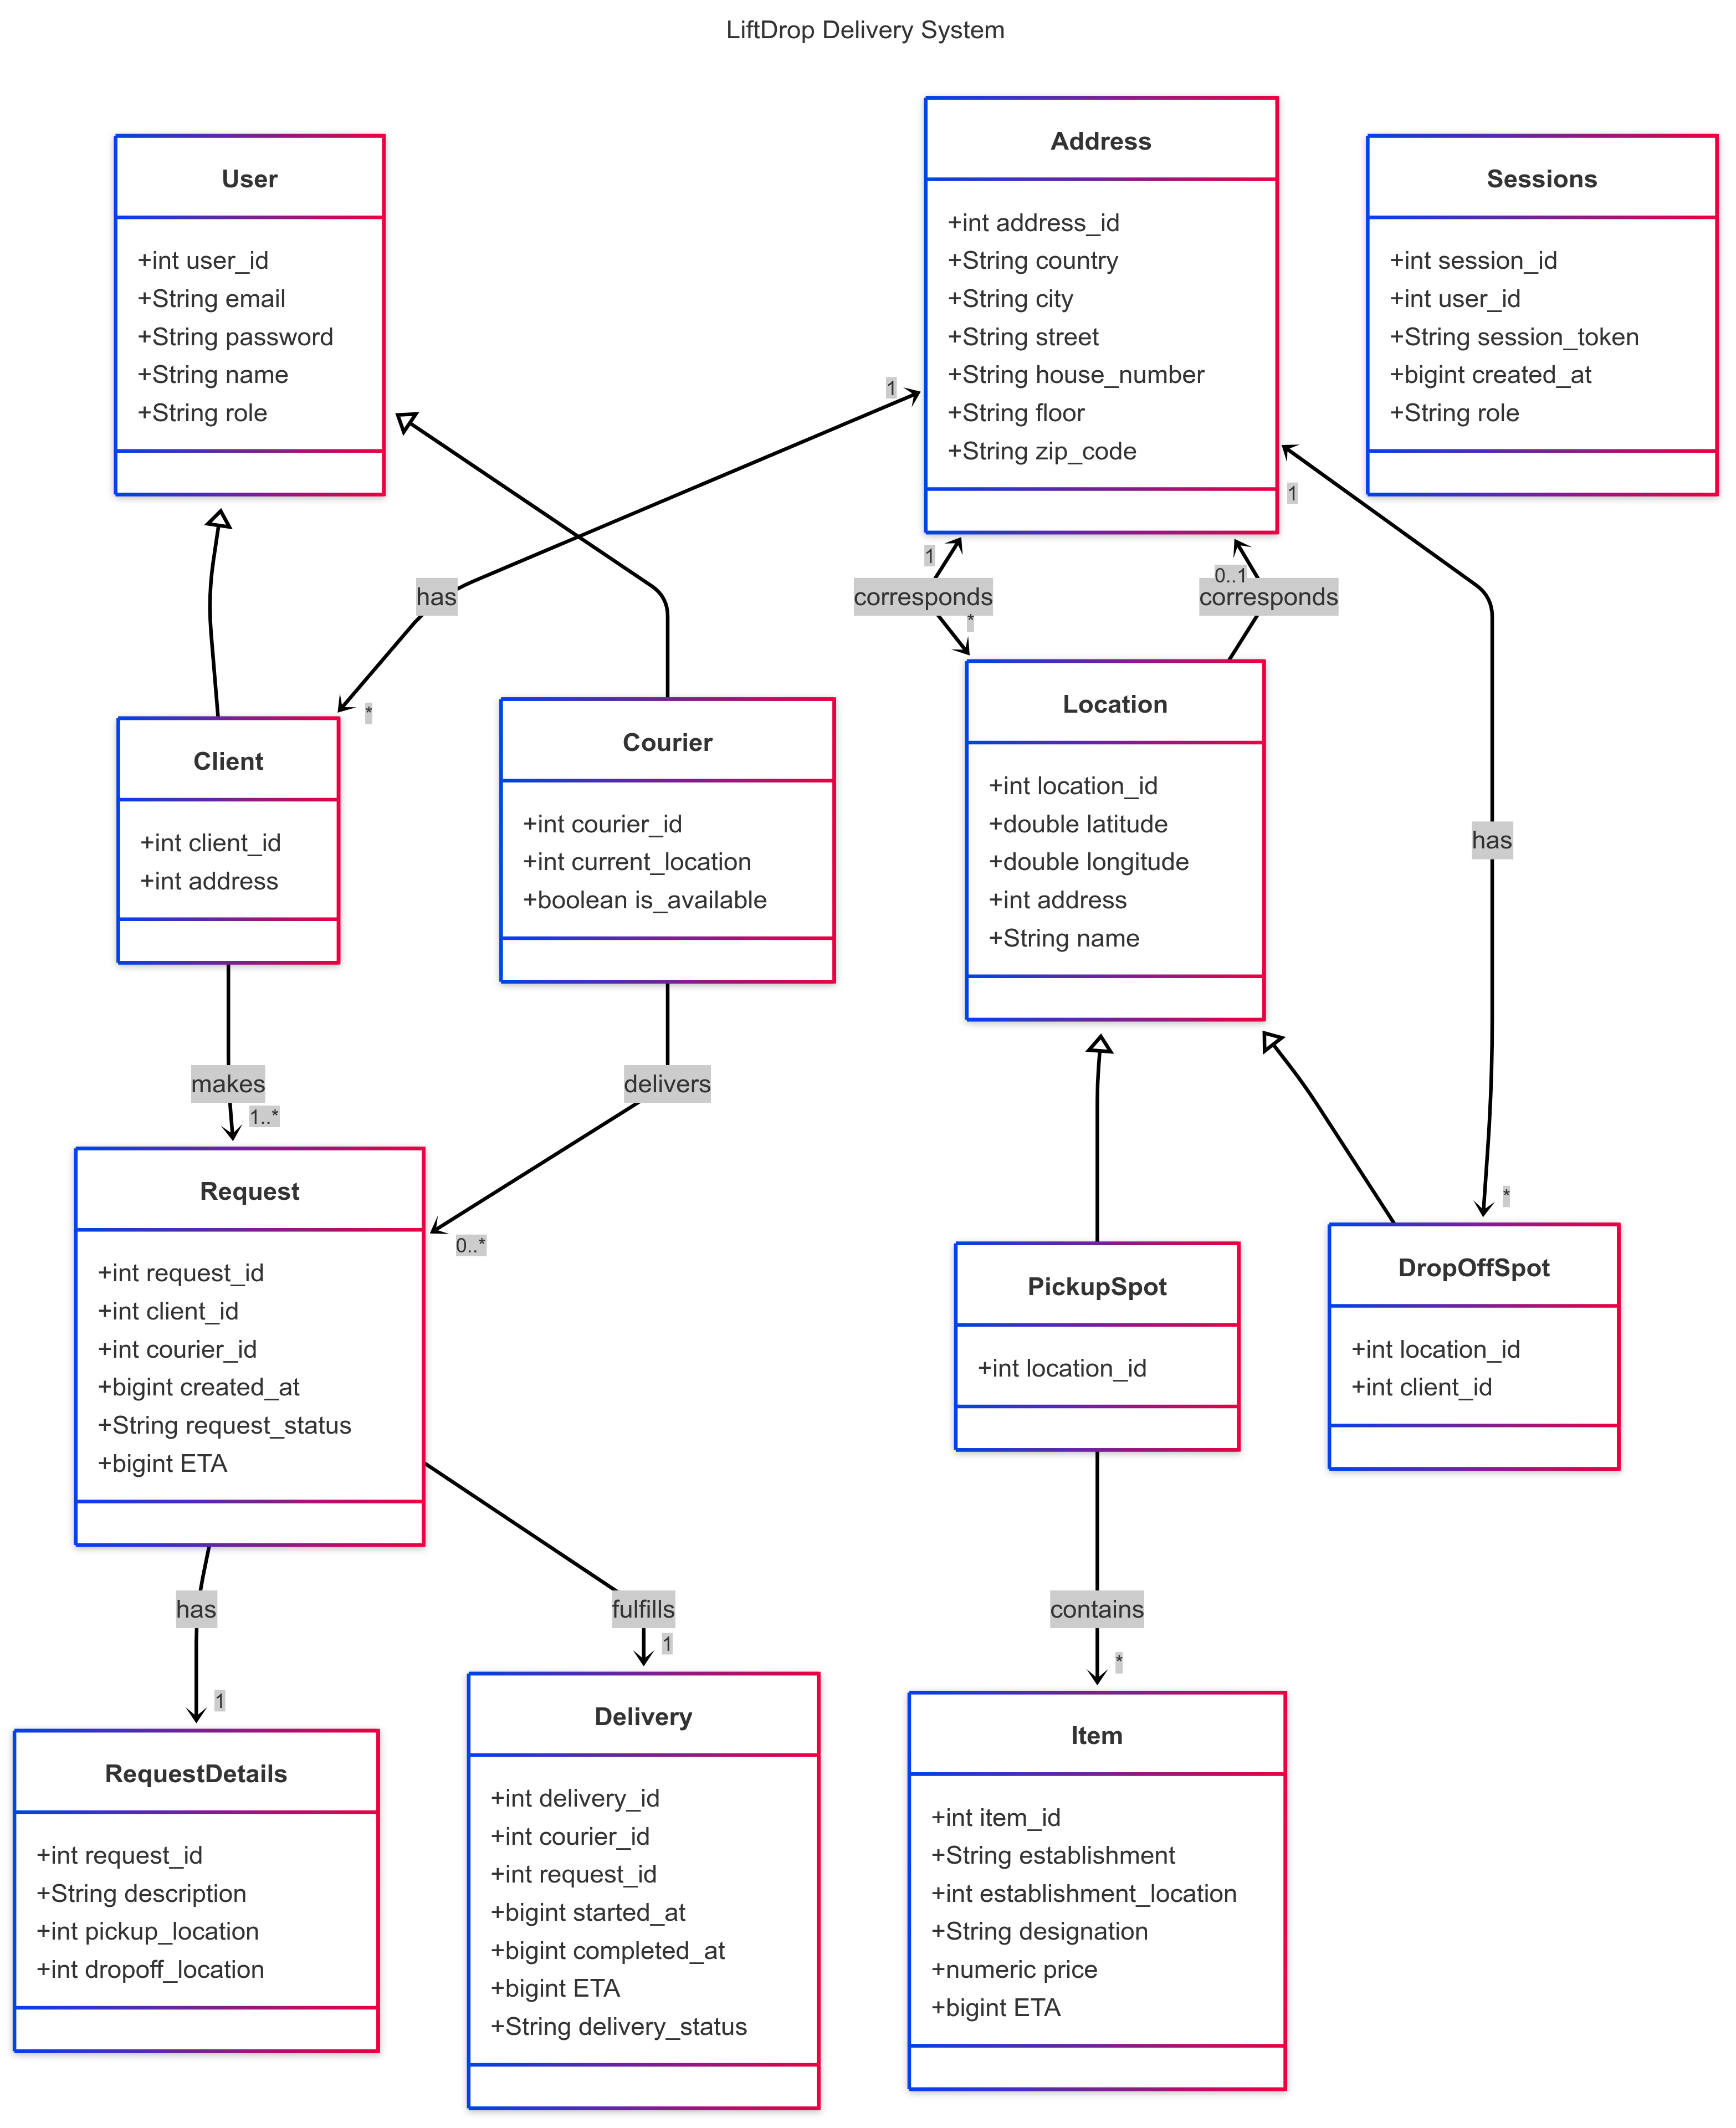
\includegraphics[width=0.8\textwidth]{images/FullDiagram.png}
    \caption{Full System Data Model}
\end{figure}

